% This must be in the first 5 lines to tell arXiv to use pdfLaTeX, which is strongly recommended.
\pdfoutput=1
% In particular, the hyperref package requires pdfLaTeX in order to break URLs across lines.

\documentclass[11pt]{article}

% Remove the "review" option to generate the final version.
\usepackage{acl}

% Standard package includes
\usepackage{times}
\usepackage{latexsym}

% For proper rendering and hyphenation of words containing Latin characters (including in bib files)
\usepackage[T1]{fontenc}
% For Vietnamese characters
% \usepackage[T5]{fontenc}
% See https://www.latex-project.org/help/documentation/encguide.pdf for other character sets

% This assumes your files are encoded as UTF8
\usepackage[utf8]{inputenc}

% This is not strictly necessary, and may be commented out,
% but it will improve the layout of the manuscript,
% and will typically save some space.
\usepackage{microtype}

% If the title and author information does not fit in the area allocated, uncomment the following
%
%\setlength\titlebox{<dim>}
%
% and set <dim> to something 5cm or larger.

\usepackage{graphicx}
\graphicspath{{../images/}}

\title{Testing Egunean Behin Visual Question Answering Dataset with BLIP}

% Author information can be set in various styles:
% For several authors from the same institution:
% \author{Author 1 \and ... \and Author n \\
%         Address line \\ ... \\ Address line}
% if the names do not fit well on one line use
%         Author 1 \\ {\bf Author 2} \\ ... \\ {\bf Author n} \\
% For authors from different institutions:
% \author{Author 1 \\ Address line \\  ... \\ Address line
%         \And  ... \And
%         Author n \\ Address line \\ ... \\ Address line}
% To start a seperate ``row'' of authors use \AND, as in
% \author{Author 1 \\ Address line \\  ... \\ Address line
%         \AND
%         Author 2 \\ Address line \\ ... \\ Address line \And
%         Author 3 \\ Address line \\ ... \\ Address line}

\author{Julen Etxaniz \\
  University of the Basque Country (UPV/EHU) \\
  \texttt{jetxaniz007@ikasle.ehu.eus}}

\begin{document}
\maketitle
\begin{abstract}
Egunean Behin is a popular Basque quiz game. The game consists on answering 10 daily multiple choice questions.
Questions were translated to English because VQA models like BLIP are mainly trained on English questions.
Three types of questions from the game were selected: figures, cubes and maze. All the images and questions were generated automatically.
There are multiple questions for each image. Questions require counting figures, colors, cubes and understanding the dimensions of the pictures.
Each question has one correct and two wrong answers. These can be used for multiple choice question answering.
\end{abstract}

\section{Introduction}

Egunean Behin is a popular Basque quiz game. The game consists on answering 10 daily multiple choice questions.
Questions were translated to English because VQA models like BLIP \cite{li2022blip} are mainly trained on English questions.
Three types of questions from the game were selected: figures, cubes and maze. All the images and questions were generated automatically.
There are multiple questions for each image. Questions require counting figures, colors, cubes and understanding the dimensions of the pictures.
Each question has one correct and two wrong answers. These can be used for multiple choice question answering.

\section{Related Work}

\subsection{Vision-language Pre-training}

Vision and language are two of the most fundamental methods for humans to perceive the world. An important goal of AI has been to build intelligent agents that can understand the world through vision and language inputs, and communicate with humans through language.

Vision-language pre-training has emerged as an effective approach to achieve this goal. Deep neural network models are pre-trained on large scale image-text datasets to improve performance on downstream vision-language tasks, such as image-text retrieval, image captioning, and visual question answering.

Models are commonly pre-trained before they are fine-tuned on each task. Fine-tuning involves additional training of the pre-trained model, using data from the downstream task. Without pre-training, the model needs to be trained from scratch on each downstream task, which leads to worse performance.

Despite the success of vision-language pre-training, existing methods have two major limitations related to models and training data.

From the model perspective, most existing pre-trained models are not flexible enough to adapt to a wide range of vision-language tasks. On the one hand, encoder-based models such as CLIP \cite{radford2021learning} and ALBEF \cite{li2021align} are less straightforward to directly transfer to text generation tasks. On the other hand, encoder-decoder models like SimVLM \cite{wang2021simvlm} have not been successfully adopted for image-text retrieval tasks.

From the data perspective, most models are pre-trained on image and alt-text pairs that are automatically collected from the web. However, these web texts often do not accurately describe the images, making them a noisy source of supervision.

\subsection{Bootstrapping Language-Image Pre-training}

To address these limitations, BLIP: Bootstrapping Language-Image Pre-training \cite{li2022blip} introduces two contributions, one from each perspective.

On the one hand, Multimodal mixture of Encoder-Decoder (MED) is a new model architecture that enables a wider range of downstream tasks than existing methods. An MED can operate either as a unimodal image or text encoder, or an image-grounded text encoder, or an image-grounded text decoder.

On the other hand, Captioning and Filtering (CapFilt) is a new dataset bootstrapping method for learning from noisy web data. A captioner model produces synthetic captions given web images, and a filter model removes noisy captions from both the original web texts and the synthetic texts.

BLIP achieves state-of-the-art performance on five vision-language tasks:  image-text retrieval, image captioning, visual question answering, visual reasoning, and visual dialog. It also achieves state-of-the-art zero-shot performance on two video-language tasks: text-to-video retrieval and video question answering.

\subsection{Visual Question Answering (VQA)}

Visual Question Answering \cite{antol2015vqa} is a popular vision and language task. Given an image and a question about the image, the task is to provide an accurate answer. VQA dataset is commonly used as a benchmark to evaluate VQA systems. Questions are generally open-ended but multiple choices are provided for some questions. If we compare it to image captioning, VQA requires a more detailed understanding of the image and more complex reasoning \cite{antol2015vqa}.

\section{Material and Methods}

This section first introduces the new model architecture MED and its pre-training objectives, then explains dataset bootstrapping and finally finetuning architecture.

\subsection{Model Architecture}

In order to pre-train a unified vision-language model with both understanding and generation capabilities, BLIP introduces a multimodal mixture of encoder-decoder (MED) model which can operate in three functionalities. The model architecture can be seen in Figure \ref{fig:blip_pretraining}.

\begin{figure*}
    \centering
    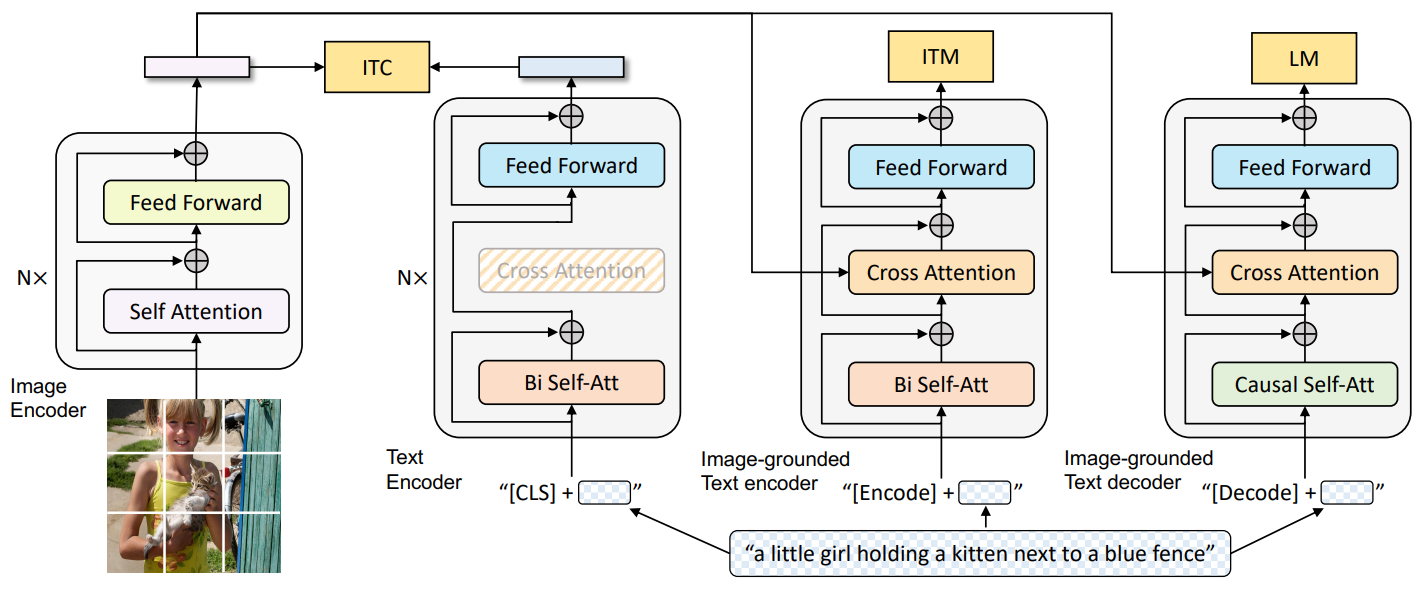
\includegraphics[width=\linewidth]{blip_pretraining.png}
    \caption{BLIP pre-training model architecture: multimodal mixture
of encoder-decoder.}
    \label{fig:blip_pretraining}
\end{figure*}

(1) Unimodal encoders are trained with an image-text contrastive (ITC) loss to align the image and text representations. The image encoder is a visual transformer \cite{dosovitskiy2020image}, which divides an input image into patches and encodes them as a sequence of embeddings. The text encoder is the same as BERT \cite{devlin2018bert}, where a \texttt{[CLS]} token is appended to the beginning of the text input to summarize it.

(2) Image-grounded text encoder is trained with a image-text matching (ITM) loss to distinguish between positive and negative image-text pairs. It has a cross-attention layer between the self-attention layer and the feed forward layer for each transformer block. The output embedding of the \texttt{[Encode]} token is used as the multimodal representation of the image-text pair.

(3) Image-grounded text decoder is trained with a language modeling (LM) loss to generate captions for given images. It replaces the bi-directional self-attention layers in the text encoder with causal self-attention layers. A \texttt{[Decode]} token is used to as the beginning of a sequence.

In order to perform efficient pre-training and improve multi-task learning, the text encoder and text decoder share all parameters except for the SA layers.

\subsection{Dataset Bootstraping}

The learning framework can be seen in Figure \ref{fig:blip_framework}.

\begin{figure*}
    \centering
    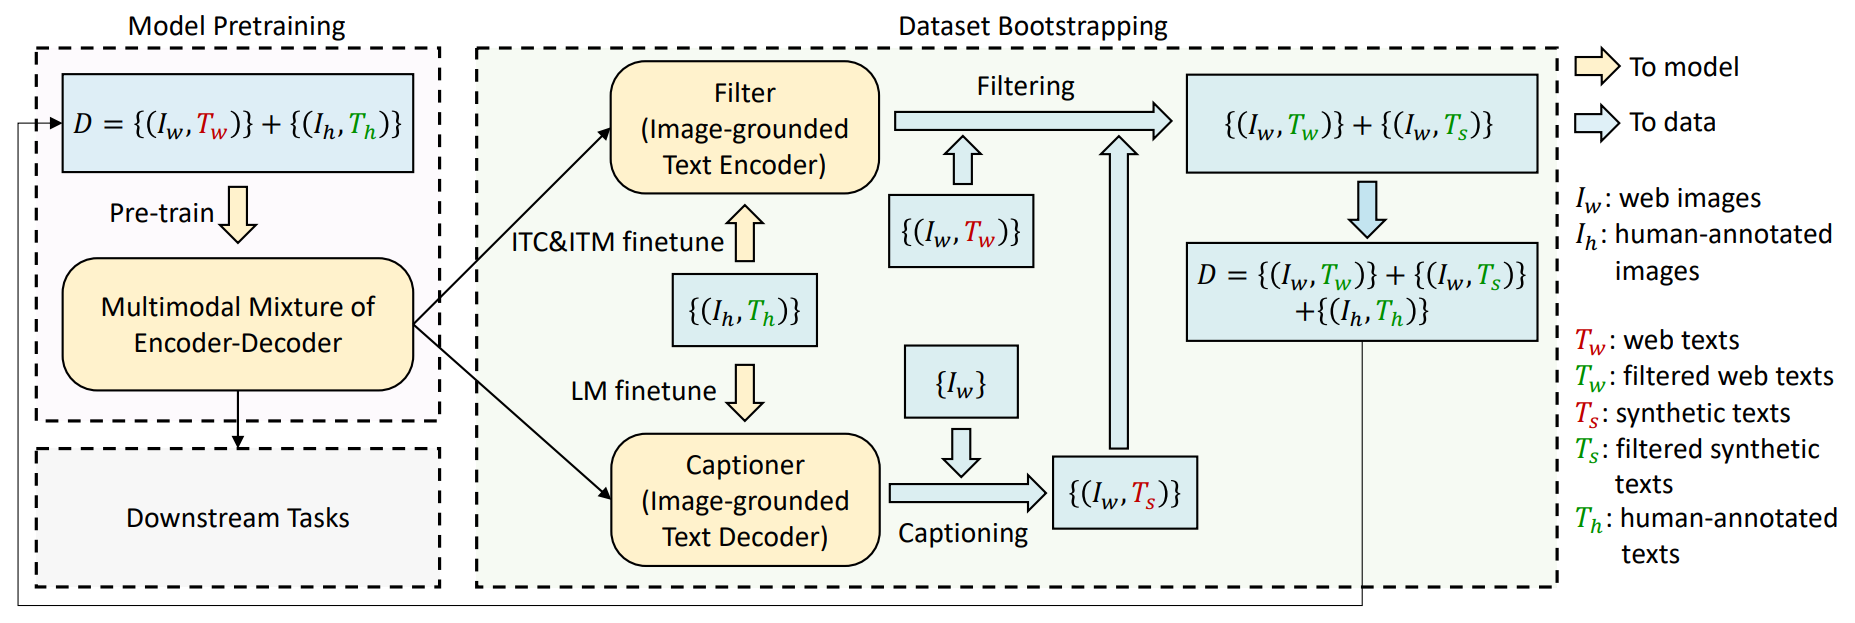
\includegraphics[width=\linewidth]{blip_framework.png}
    \caption{BLIP learning framework: a captioner to produce synthetic captions and a filter to remove noisy captions.}
    \label{fig:blip_framework}
\end{figure*}

\subsection{Finetuning}

On different downstream tasks, different paths of the pre-trained model are finetuned to achieve different objectives. The finetuning architecture for VQA can be seen in Figure \ref{fig:vqa_example}.

\begin{figure*}
    \centering
    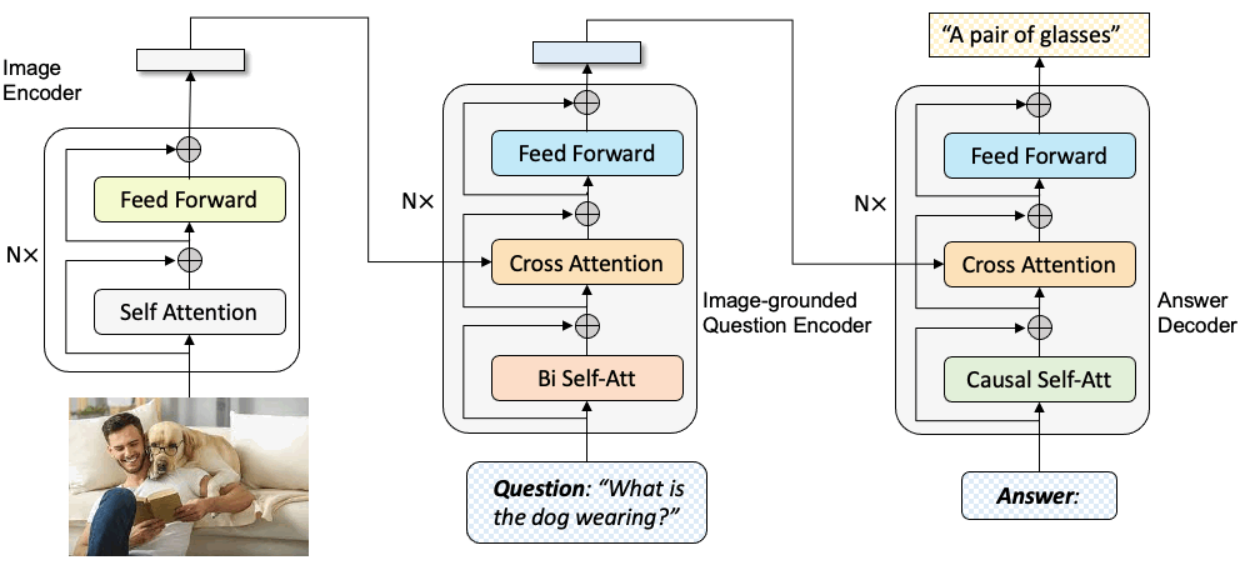
\includegraphics[width=\linewidth]{vqa_example.png}
    \caption{BLIP VQA finetuning architecture.}
    \label{fig:vqa_example}
\end{figure*}

\section{Results}

\section{Conclusions}

\bibliography{egunean_behin_vqa}
\bibliographystyle{acl_natbib}

\end{document}
